\documentclass[a4paper,man,floatsintext,natbib,donotrepeattitle]{apa6}

\usepackage[english]{babel}
\usepackage[utf8x]{inputenc}
\usepackage{amsmath}
\usepackage{graphicx}
\usepackage[colorinlistoftodos]{todonotes}
\usepackage{natbib}
\usepackage{subcaption}
\usepackage{pdfpages}
\usepackage{hyperref}
\usepackage{comment}

\hypersetup{
	colorlinks=true,
	linkcolor=black,
	citecolor=black,
	urlcolor=black
}

\definecolor{Blue}{RGB}{0,0,255}
\definecolor{Green}{RGB}{10,200,100}
\definecolor{Red}{RGB}{255,0,0}
\definecolor{Orange}{RGB}{255,140,0}
\definecolor{White}{RGB}{255,255,255}
\newcommand{\jd}[1]{\textcolor{Blue}{[jd: #1]}}  
\newcommand{\ek}[1]{\textcolor{Orange}{[ek: #1]}} 
\newcommand{\hideref}[1]{\textcolor{White}{[refs: #1]}} 

\newcommand{\subsubsubsection}[1]{{\em #1}}
\newcommand{\eref}[1]{(\ref{#1})}
\newcommand{\tableref}[1]{Table \ref{#1}}
\newcommand{\figref}[1]{Figure~\ref{#1}}
\newcommand{\appref}[1]{Appendix \ref{#1}}
\newcommand{\sectionref}[1]{Section \ref{#1}}

%\title{TITLE}
\shorttitle{Supplementary Material: Norming Studies}
%\author{Elisa Kreiss} 
%\affiliation{Osnabrueck University}

\begin{document}

\pagenumbering{Roman}

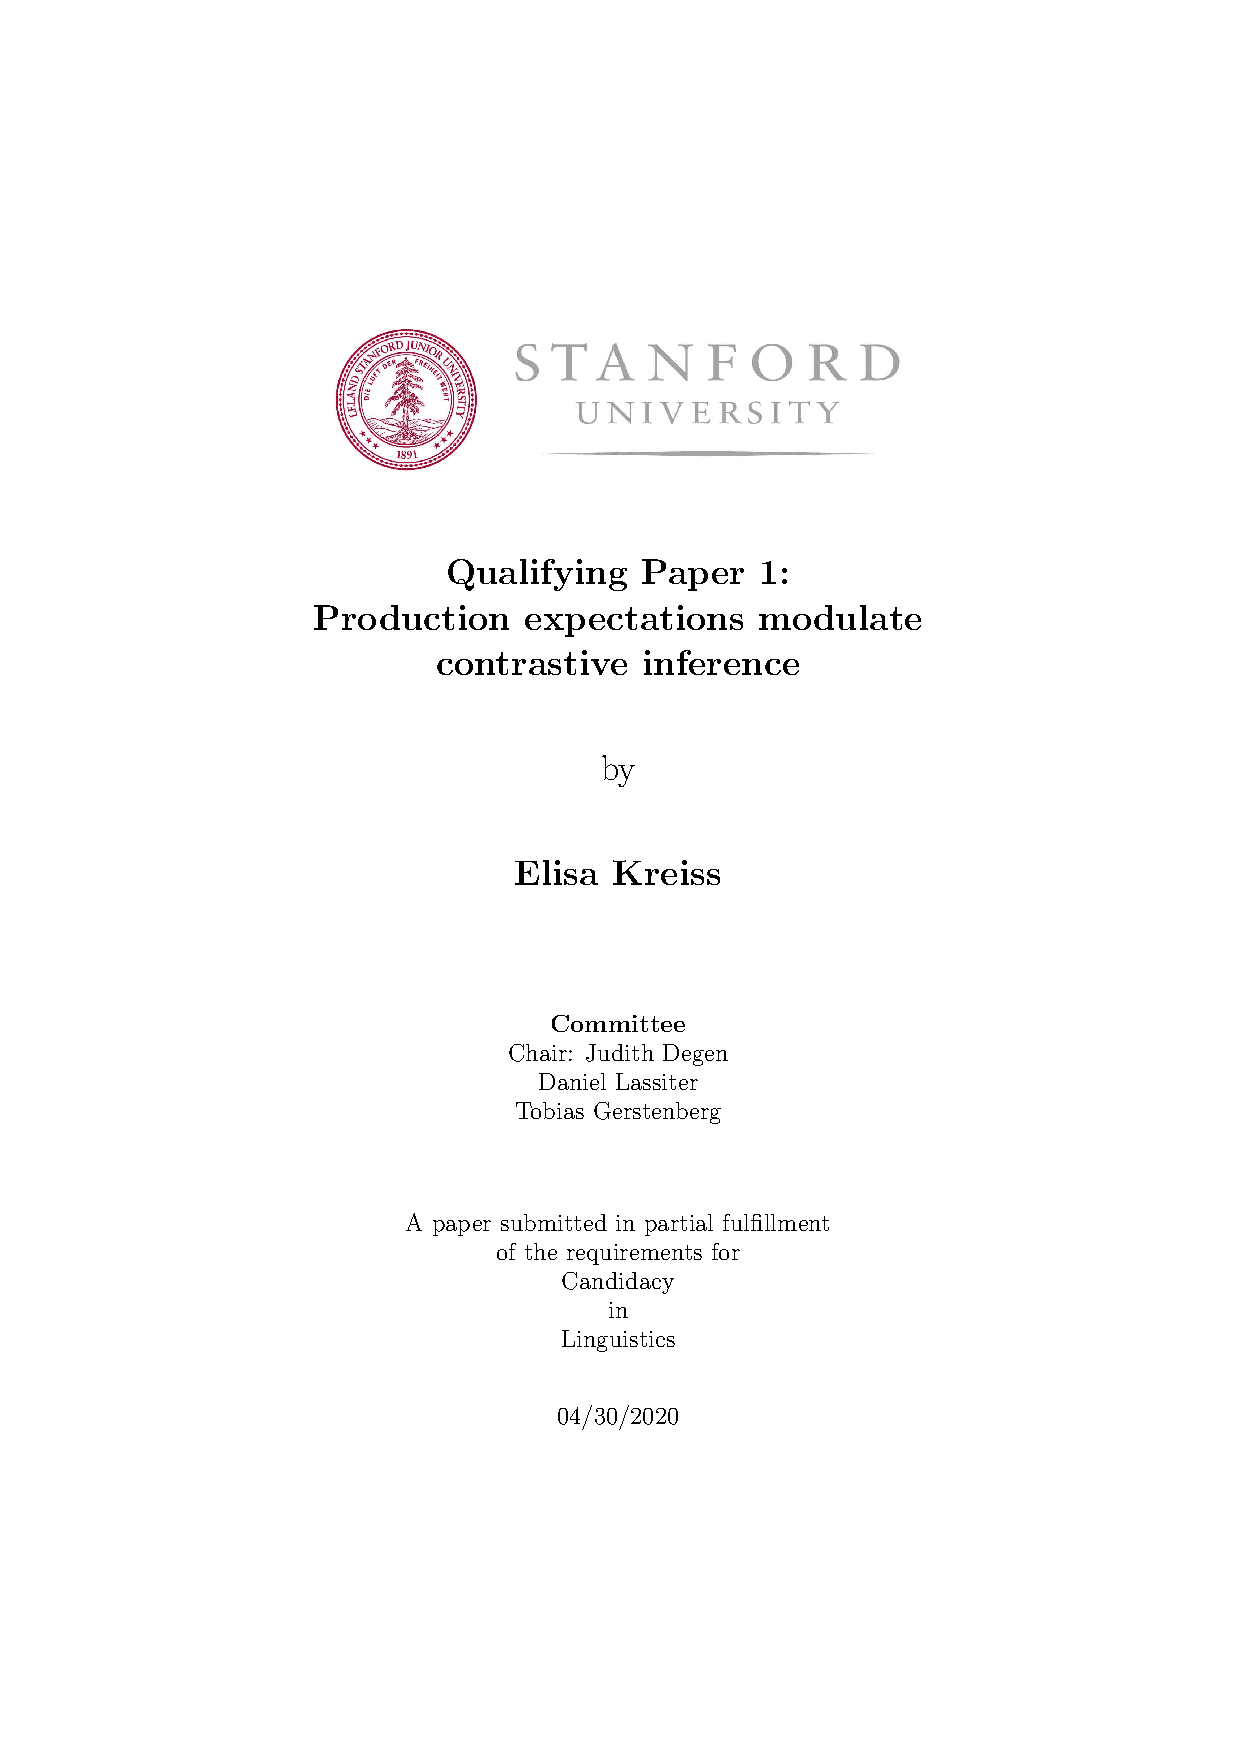
\includepdf[pages={1}]{titlepage/titlepage.pdf}

% 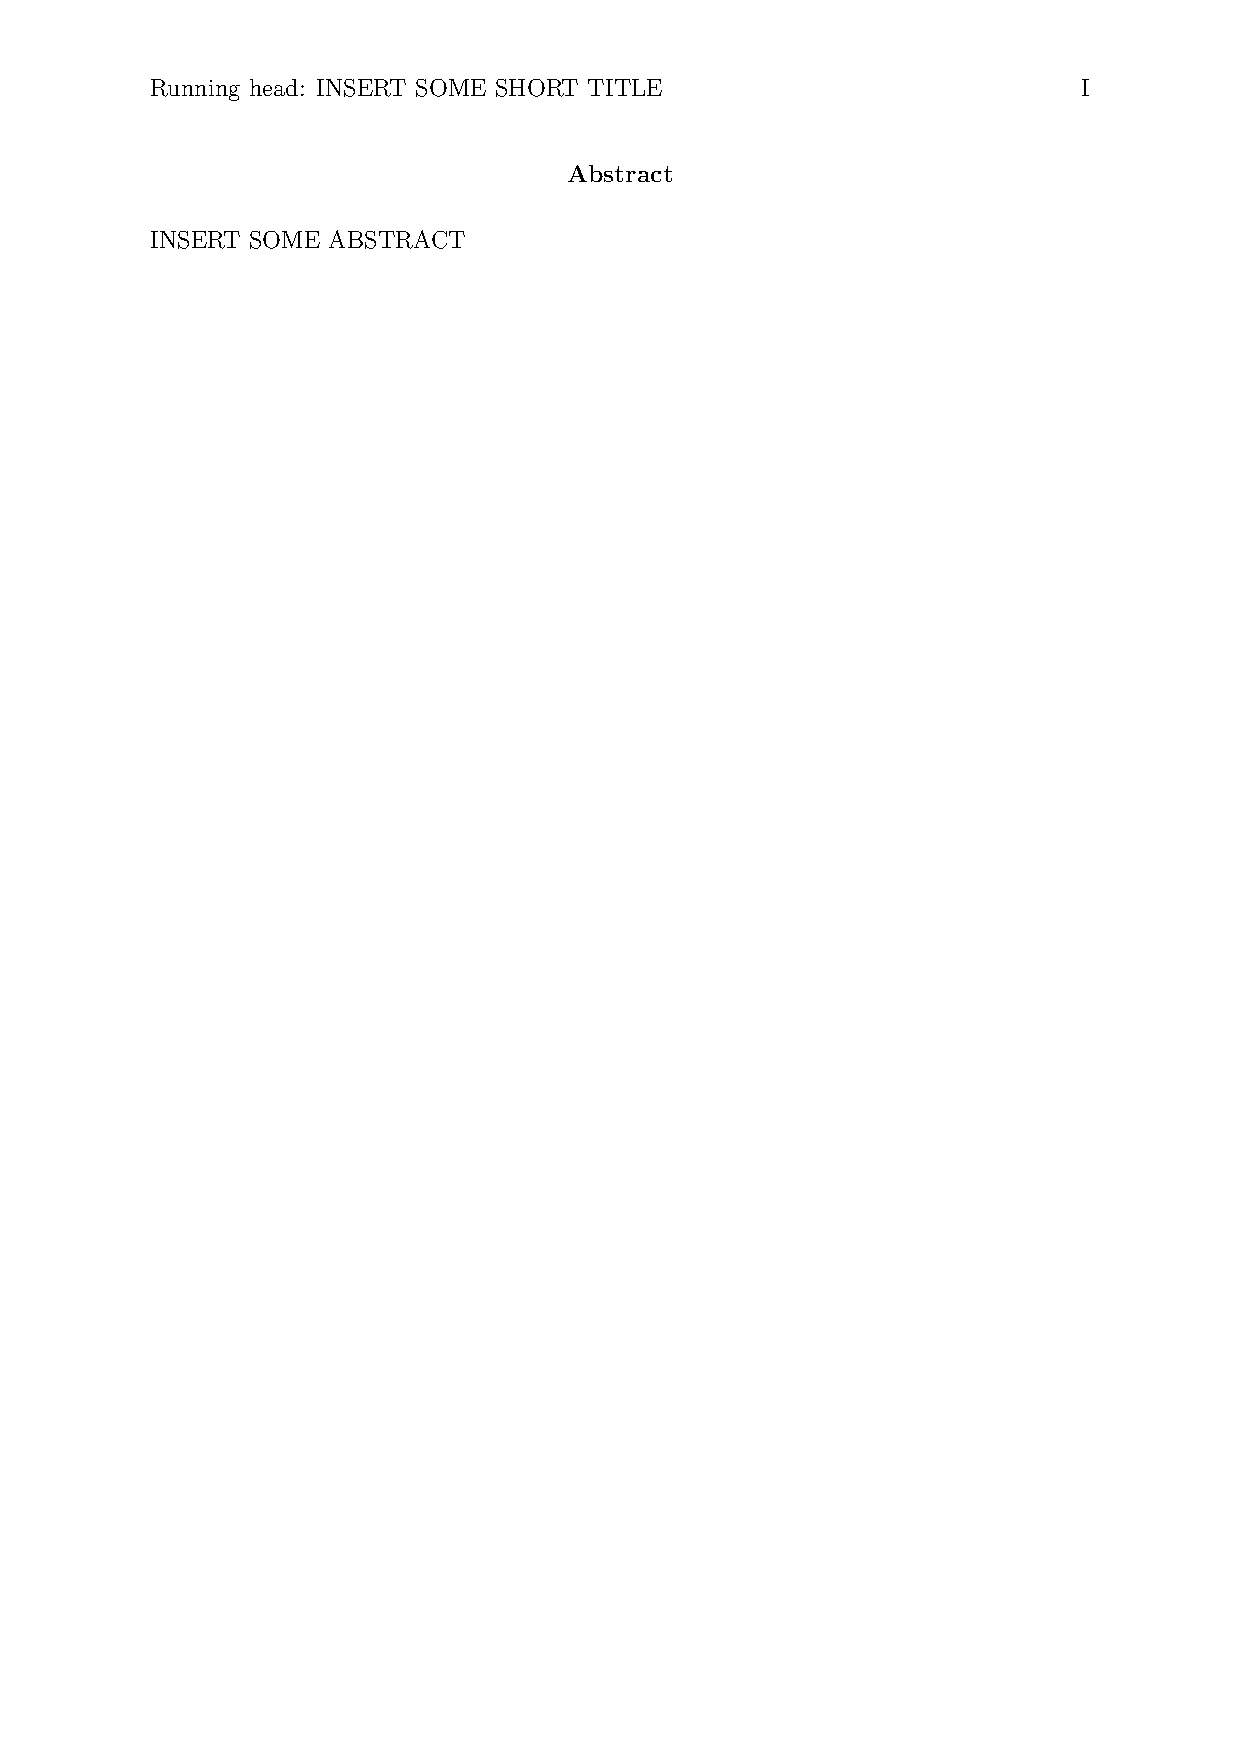
\includepdf[pages={1}]{abstract/abstract.pdf}

\clearpage

%{\def\addcontentsline#1#2#3{}}
\setcounter{page}{2}
\tableofcontents

\setcounter{secnumdepth}{3}

\clearpage

% \ek{watch your tenses; define a common textit/quotation style}

\pagenumbering{arabic}
\setcounter{page}{1}

% \section{Introduction}
% \subsection{SOME SUBSECTION}\label{sec:somesubsection}

% \section{Experiment: Norming} \label{experiment}

% We want to manipulate the modifier production probabilities a listener can expect for an object in isolation. In other words, we want to manipulate whether the listener rather expects a speaker to use a modified referring expression, such as ``the curvy/small/yellow banana'' or the unmodified expression ``the banana''. For that purpose, we chose an adjectival domain where those production probabilities can be easily manipulated, namely color modifiers. First of all, color modifiers are more likely to be used for an object in isolation (i.e., redundantly) than other adjective types \citep{Pechmann:1982}. Furthermore, their use is not arbitrary but dependent on the noun they modify \citep{Tanaka:1999,Sedivy:2003}. If one particular color is a defining property for the object, the object is \textit{color-diagnostic} and speakers only very rarely use the color modifier redundantly to refer to it \citep{Tanaka:1999}. Color-diagnostic objects are for example bananas, which are generally associated with the color yellow. Cups on the other hand are non-color-diagnostic objects, since they are not associated with one particular color and color itself is not a perceptual property that defines it. Even though a sports car is primarily associated with the color red, color itself is not a defining perceptual property of the object, which is why it is also considered a non-color-diagnostic object \citep{Tanaka:1999}. 

% Although color-diagnostic objects are rarely modified redundantly when they occur in their typical color, they often are when they occur in an atypical color instead. For example, a yellow banana is mainly referred to as ``a banana'', while a blue banana is referred to as ``a blue banana'' \citep{Westerbeek:2015}. To manipulate the modifier production probabilities a listener can expect, we therefore use typical and atypical instances of color-diagnostic objects.

\section{Desiderata for experimental items}

% Judith: Here and elsewhere, rather than framing it from the perspective of "what we wanted to do" (because it doesn't make clear *why* we "wanted" to do that), frame it from the perspective of what the requirements on the stimuli were. I'd suggest having a separate section before you get into each of the experiments that's entitled sth like "Desiderata for experimental items", in which you say what was required of the stimuli. You can take as given what is said in the main text and focus on what the important properties were that you normed for (and why those properties were important)

Manipulating the typicality of color-diagnostic items for an experiment in the contrastive inference paradigm posited a number of requirements onto the items. 
% To determine the most suitable items, a variety of objects was carefully normed and only a subset was selected for the final set of stimuli. 
First of all, the objects needed to be color-diagnostic (Section \ref{coldiagnorming}), since those objects show the highest difference in color modifier use dependent on their color typicality \citep{Westerbeek:2015,Tanaka:1999,Sedivy:2003}, our central manipulation. In addition, the items needed to be shape-diagnostic, such that they would still be recognizable when presented in a non-prototypical color. Plums, oranges, limes and lemons for example are objects with low shape-diagnosticity and are therefore hard to identify when presented in an atypical color (Section \ref{freeprodnorming}). Furthermore the items needed to be easily recognizable and nameable (Section \ref{nameabilitynorming} and \ref{freeprodnorming}). Previous literature suggests that unexpected utterances and labels might be a confound in eyetracking experiments \citep{Qing:2018}. To make the items further suitable for eyetracking studies, target and color competitor were never cohort competitors of each other (e.g., \cite{Cole:1980}, \cite{Marslen-Wilson:1984}), i.e., they were always distinguishable at noun onset.

Furthermore, to our knowledge, previous experiments which manipulated the color typicality of objects did not counterbalance the colors used for typical and atypical instances. Certain colors (e.g., blue) primarily occurred as an atypical instance while other colors (e.g., green) occurred as a typical one. However, color hues vary in their a priori preference and elicit different emotional responses (see \cite{Palmer:2013, Elliot:2014} for reviews on color preference and psychology). The color hue imbalance for typical and atypical objects might therefore be a non-negligible confound to the typicality effect. Each color in our data set occurs twice as a typical instance and twice as an atypical instance to counteract this potential confound.

Finally, the typical and atypical instance of each object was normed to ensure that the color manipulation of the images shows the desired difference in typicality ratings (Section \ref{typicalitynorming}).

Since half of the conditions require the target and color competitor both to be (a)typical, we needed two (a)typical instances for each color. Motivated through this experimental design, the final set of stimuli consists of ten color diagnostic objects (each of them in a typical and atypical instantiation), evenly distributed over five colors. To determine the most suitable items, our initial set of potential stimuli comprised six colors (green, orange, pink, red, white, yellow), each with at least four presumably typical color-diagnostic instances (25 items in total).

\section{Norming for color-diagnosticity}
\label{coldiagnorming}
% List feature norming

% Goal: determine color diagnosticity
% (1) Is color a property that is closely associated with the object?
% (2) If a color is mentioned, do participants agree on the color?

% Task: "List 3 perceptual features of a \textbf{NOUN}"

% free production and checkbox with possibility to say "I don't know this object."

% 52 trials;
% 4 control trials with nonce words;
% 25 presumably color diagnostic objects (4 for each of the 6 colors + 1 more green thing) and 23 presumably non-color diagnostic objects

% 40 participants;
% exclusion criteria: everyone correctly identified the 4 nonce words as unknown objects; and if they rated more than 8 objects as "object unknown" they were excluded (2 participants);
% resulting number of participants: 38

% we evaluated the results according to whether 
% (1) a color was mentioned at all in the features
% (2) a color was mentioned as a first feature
% (3) if a color was mentioned, was it the same or did they differ

All potential stimuli were normed for their color-diagnosticity. Items were considered color-diagnostic if color was a perceptual property that was closely associated with the object, and if there was agreement on the specific color it was associated with \citep{Tanaka:1999}.

\paragraph{Participants}
We recruited 40 participants over Amazon's Mechanical Turk. We restricted participation to workers within the US and a previous Hit approval rate of at least 98\%. The study took about 20 minutes and we paid \$4.00 for participation. All participants indicated that their native language was English.

\paragraph{Materials and procedure}

\begin{figure}
	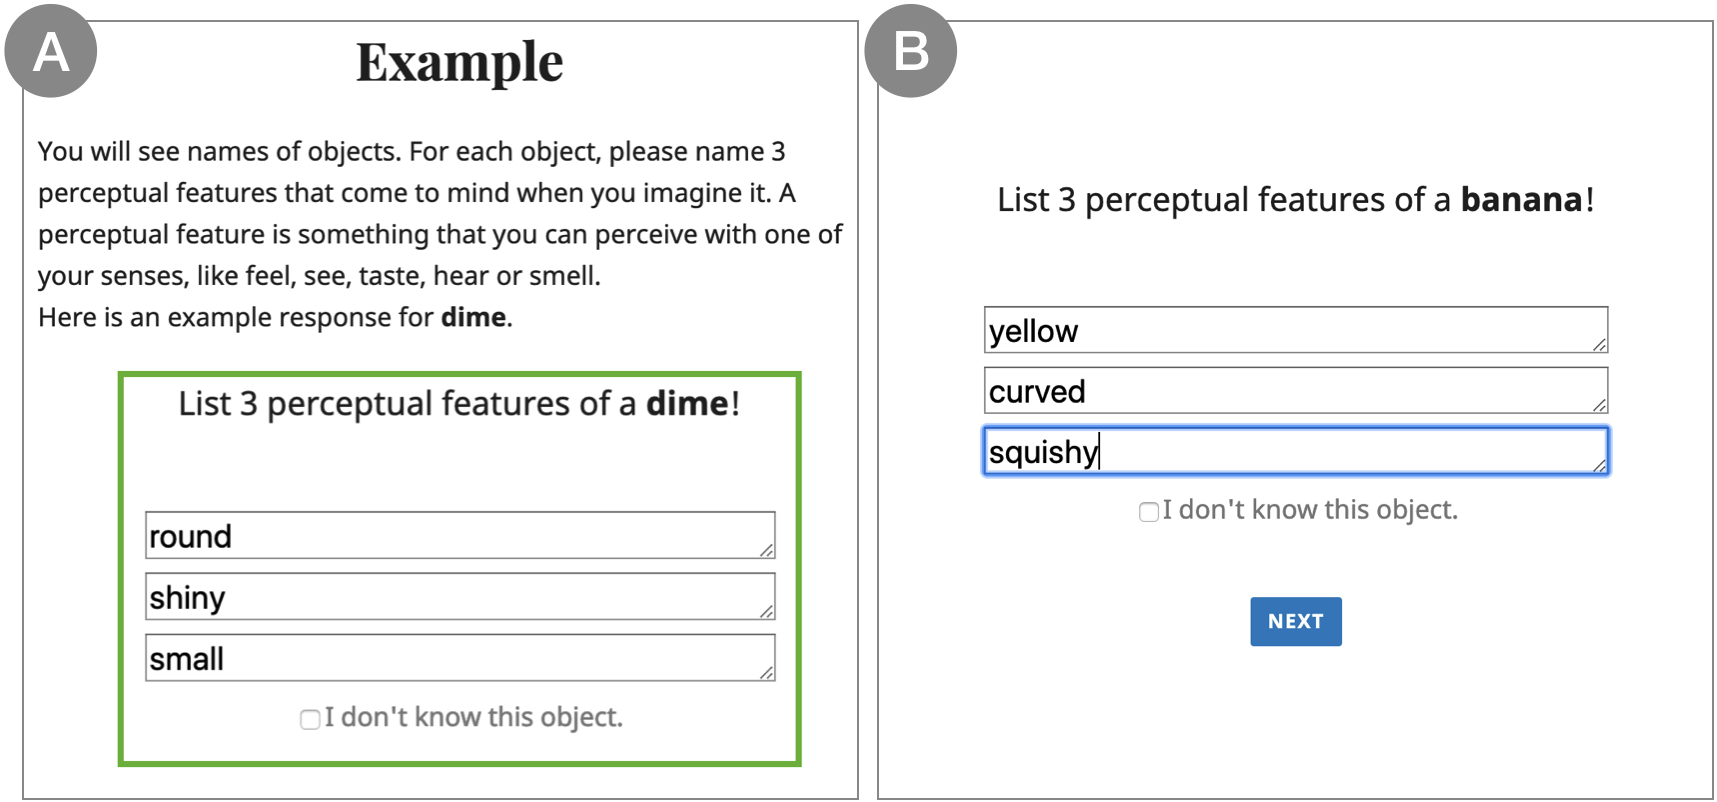
\includegraphics[width=\linewidth]{img/norming1_design.png}
	\caption{Example trial (in A) and critical trial (in B) for the color-diagnosticity norming experiment.}
	\label{fig:norming1design}
\end{figure}

The experimental design is adapted from \cite{Tanaka:1999}. 
Participants were asked to list three perceptual features of an object, which they entered into three free production text boxes. They could proceed to the next trial if they either entered all three features or indicated by ticking a checkbox that they did not know the object. In the beginning of the experiment, participants saw an example trial where the term \textit{perceptual feature} was defined and they were shown an example response for the object \textit{dime}, which was described as \textit{round}, \textit{shiny}, and \textit{small} (as used in \cite{Tanaka:1999}).

Each participant saw 52 trials, four of which were control trials with nonce words. From the remaining trials, 25 asked for presumably color-diagnostic objects (four for each of the six colors and one additional green object), and 23 asked for presumably non-color-diagnostic objects. The example trial and one of the critical trials is displayed in Figure \ref{fig:norming1design}.

\paragraph{Analysis and exclusions}
All participants indicated that they were unfamiliar with the four nonce words we had included as attention checks. Two participants were excluded because they rated more than eight objects as unknown to them, resulting in a total of 38 participants.

\paragraph{Results}
An item was considered color-diagnostic if color was mentioned as the first feature, \textbf{and} participants agreed on the specific color the object was associated with. 
% The goal was to find 10 highly color-diagnostic objects spread evenly over five colors (i.e., two objects in each color).

\begin{figure}
	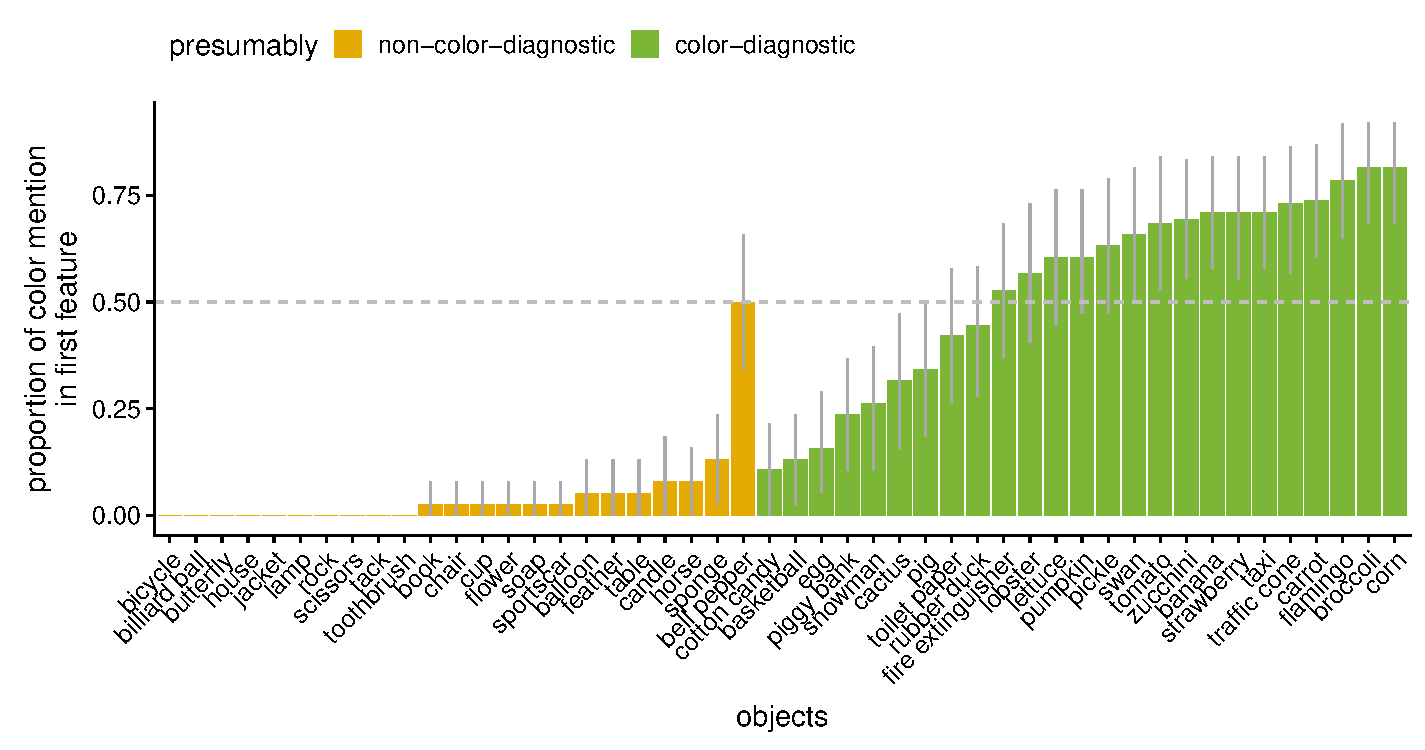
\includegraphics[width=\linewidth]{img/norming1_resultsoverall.pdf}
	\caption{Proportion of color being mentioned as a first perceptual feature for presumably non-color-diagnostic objects (orange) and color-diagnostic objects (green). Color was generally mentioned more often for the color-diagnostic objects. An exception to that is bell pepper, which is categorized as non-color-diagnostic because it is associated with more than one color.}
	\label{fig:norming1resultsoverall}
\end{figure}

As expected, color was in general more likely to be mentioned for the objects that were intended to be color-diagnostic and less likely for the non-color-diagnostic objects (see Figure \ref{fig:norming1resultsoverall}). An exception to that was \textit{bell pepper} which was expected to be non-color-diagnostic but for which participants still mentioned color as an important perceptual feature. However \textit{bell pepper} was associated with more than one color. Although it was mainly described as \textit{green}, several participants also mentioned \textit{red} and to a small degree \textit{black}, \textit{yellow} and \textit{orange}. 
For all items that were intended to be color-diagnostic, participants generally agreed on the color. 

\begin{figure}
	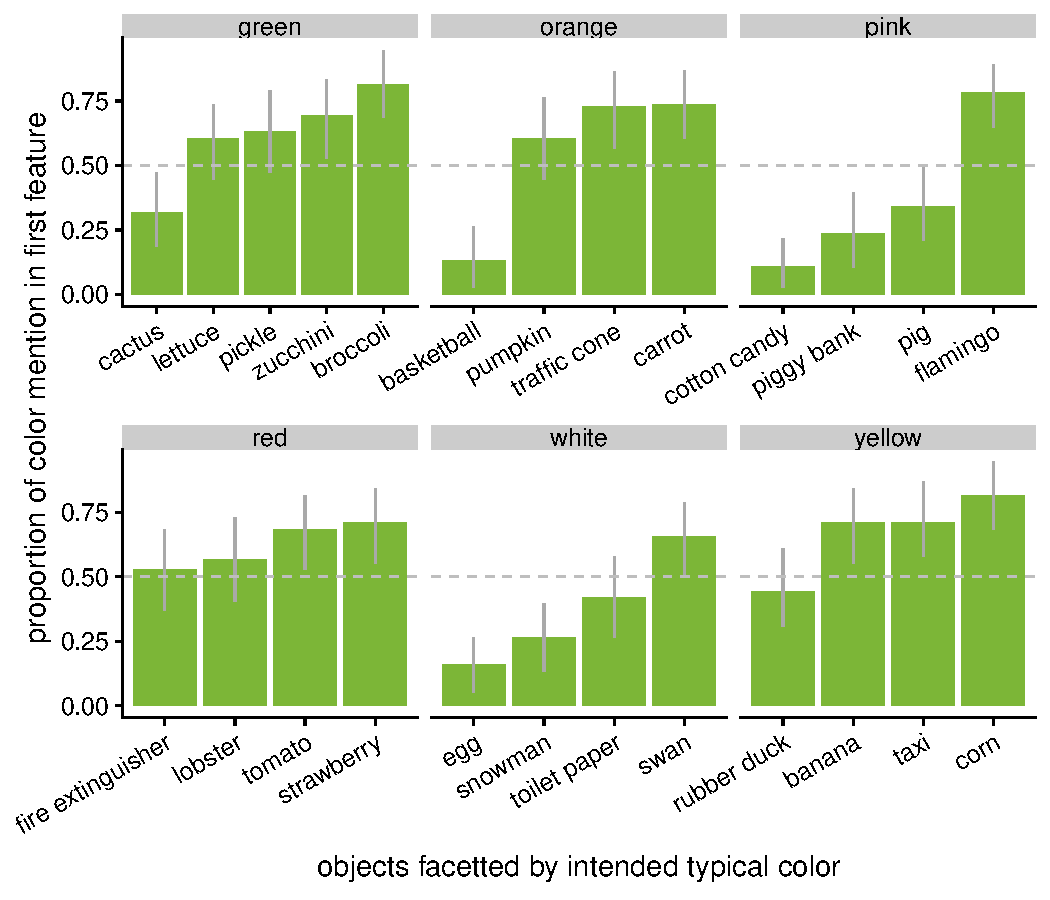
\includegraphics[width=0.75\linewidth]{img/norming1_results.pdf}
	\caption{Proportion of color being mentioned as a first perceptual feature for presumably color-diagnostic objects, facetted by the assumed color association. The dotted line marks the point where half of the time, color was mentioned as the first feature.}
	\label{fig:norming1results}
\end{figure}

Figure \ref{fig:norming1results} shows the proportion of color mention as the first perceptual feature, facetted by the color they were associated with. The dashed horizontal line marks the case when color was mentioned half of the time as the first perceptual feature. The items in the colors pink and white had the lowest proportion of color mention overall. This is the main reason why pink items were excluded from the final set of stimuli. Items with low proportions of color mention in each color were less likely to be chosen as stimuli, which is why we for example excluded \textit{cactus}, \textit{basketball} and \textit{cotton candy} from the final set. 


\section{Norming for nameability}
\label{nameabilitynorming}

% Goal: Are the image depictions we chose nameable, the way we intended?

% Task: "What is this?"

% free production

% 50 trials;
% 26 depictions of presumably color diagnostic objects (same as in color diagnosticity norming + 1 more lettuce depiction) and 24 presumably non-color diagnostic ones (same as in color diagnosticity norming + 1 more (sports)car);

% 20 participants;
% exclusion: 2 participants because they indicated that they were confused or didn't do the HIT correctly;
% resulting number of participants: 18

% We evaluated the results according to how many labels were used. If more than one label was used, we favored cohort competitors over entirely separate terms (e.g., bike and bicycle are more acceptable than traffic cone and cone);
% Wrt to lettuce we had romaine and iceberg lettuce depictions. The simple noun lettuce was more frequently used for the iceberg than the romaine lettuce which is why we favored the iceberg lettuce.; 
% other things: zucchini was half of the time misclassified as cucumber, similarly for pickle, traffic cone had a lot of different labels, such as simply cone, caution cone, hazard cone, safety cone

After we normed for color-diagnosticity, we chose an image depiction for each object and normed them for their nameability. Determining whether an object is nameable served two main purposes. Firstly, we ensured that the dominantly chosen label corresponds to the concept we had normed for in the color-diagnosticity norming (Section \ref{coldiagnorming}). Furthermore, participants should agree on the label that best describes the chosen depiction. Strong agreement among participants is an indication that the noun label can be used reliably. Strong disagreement about the label might affect the production and comprehension of the referring expressions. If speakers are uncertain about an object's property (in this case, its type), they are more likely to overmodify \citep{Horacek:2005, Williams:2017}. Additionally, a listener's surprisal of hearing an unexpected label might affect for instance their fixations in eyetracking experiments, creating a potential confound in the analysis \citep{Qing:2018}.

\paragraph{Participants}
We recruited 20 participants over Amazon's Mechanical Turk. We restricted participation to workers within the US and a previous Hit approval rate of at least 97\%. The study took about 7 minutes and we paid \$1.30 for participation. All participants indicated that their native language was English.

\paragraph{Materials and procedure}

\begin{figure}
	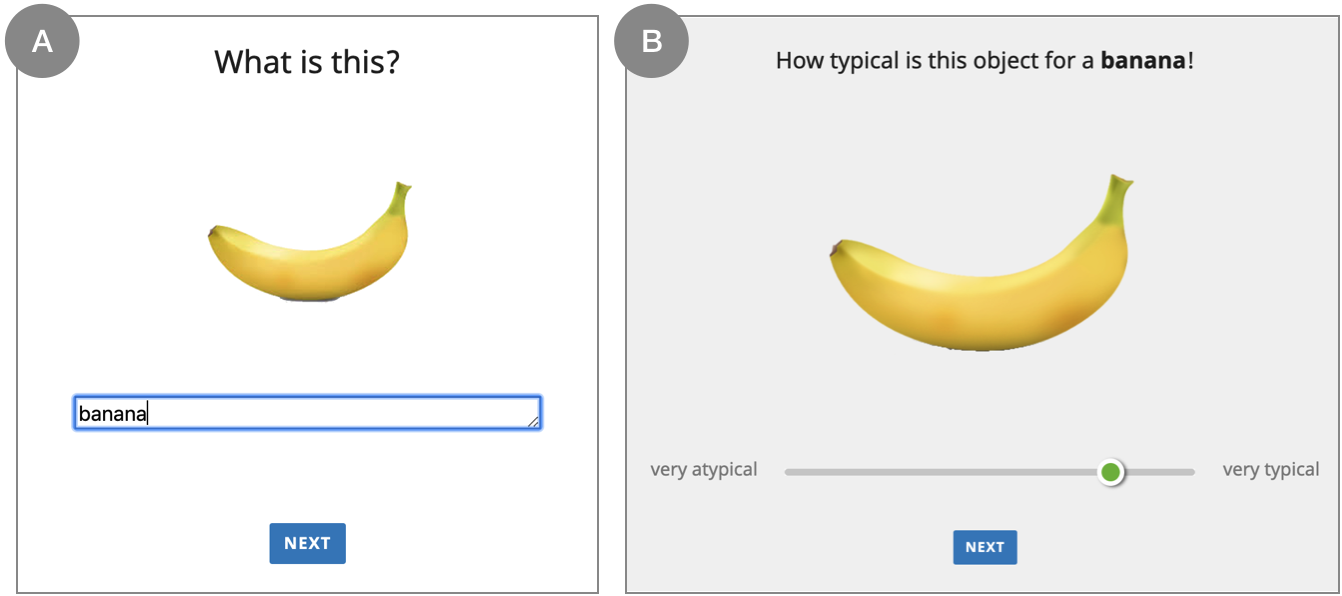
\includegraphics[width=\linewidth]{img/norming2and3_design.png}
	\caption{Example trials of nameability and free production norming (in A) and typicality norming (in B).}
	\label{fig:norming23design}
\end{figure}

Each participant saw 50 trials in which they were asked ``What is this?'' with a depiction of an object and a free production text field, as shown in Figure \ref{fig:norming23design}A.
We used the same objects as in the color-diagnosticity norming study (i.e., 25 color-diagnostic and 23 non-color-diagnostic objects). In two cases (lettuce and sports car) we chose two depictions to determine the most prototypical instance of these items.

\paragraph{Exclusions}
Two participants were excluded because they indicated that they might have misunderstood the instructions, resulting in a total of 18 participants.

\paragraph{Results}
We evaluated the results according to how many labels were used. If more than one label was used, we favored cohort competitors (e.g., \textit{bike} and \textit{bicycle} were more acceptable deviations than \textit{traffic cone} and \textit{cone}).

Overall, participants agreed on the labels, but there were some notable exceptions. Both, the pickle and zucchini, were called \textit{cucumber} to a non-negligible degree. Given that they also have low shape-diagnosticity, both objects were excluded from the final set of stimuli. Other items that received a variety of labels were the traffic cone (e.g., \textit{traffic cone, cone, caution cone, hazard cone}) and the rubber duck (e.g., \textit{rubber duck, duck, duck toy}). These cases were problematic because the labels are not cohort competitors of each other, which makes them crucially distinct in real-time (auditory) setups such as eyetracking experiments. 

Finally, we investigated which depiction best represented the generic lettuce: romaine or iceberg. We found that when participants saw the iceberg lettuce before the romaine lettuce, they simply called it \textit{lettuce}. However, if they saw the romaine lettuce first, they called it \textit{romaine lettuce} 20\% of the time. This suggests that the iceberg lettuce is the more prototypical lettuce (in the MTurk community) and was therefore chosen for the final set of stimuli. 


\section{Norming for typicality}
\label{typicalitynorming}

% Goal: Does the color manipulation of the images show the desired difference in typicality ratings?

% Task: "How typical is this object for a \textbf{NOUN}?"

% slider rating, underlyingly coded as ranging from 0 to 100

% 45 trials;
% 11 color diagnostic objects, each in their typical color and 1-2 atypical colors (i.e., 25 stimuli); 20 non-color diagnostic stimuli

% 30 participants;
% exclusions: none; everyone thought they did the HIT correctly

% Results: generally clear distinction between typical and atypical instance;
% From the three items that were normed in two atypical colors (carrot, corn, pumpkin), we see the biggest difference between the red and white pumpkin. Therefore, we should choose the white pumpkin and (following from that) the green carrot and red corn.
% There does not seem to be a big difference between the yellow egg and snowman, but the white egg is rated even more typical and its size fits better to the other stimuli. Therefore, we should choose the egg over the snowman (given that both are also nameable).
% Even though the orange banana is predominantly rated below 50, it is still not as atypical as other objects.
% The non-color diagnostic objects are all rated as very typical instances.

After selecting the most promising objects and creating atypical counterparts, we normed depictions of these items according to their typicality to ensure that they are in fact perceived as typical and atypical. Norming the atypical instances is especially necessary since in fact most of these items occur in different colors in the world. For example, there are red bananas, purple carrots, blue corn cobs, yellow tomatoes, varying colors of pumpkins and artificially colored eggs. A successful typicality manipulation should maximize the difference between typical and atypical ratings for each object.

\paragraph{Participants}
We recruited 30 participants over Amazon's Mechanical Turk. We restricted participation to workers within the US and a previous Hit approval rate of at least 97\%. The study took about 4 minutes and we paid \$0.80 for participation. All participants indicated that their native language was English.

\paragraph{Materials and procedure}
Each participant saw 45 trials in which they were asked ``How typical is this object for a \textbf{NOUN}'' with a depiction of an object in either its typical or atypical instance, as shown in Figure \ref{fig:norming23design}B, and where \textbf{NOUN} is the established label from the nameability norming experiment. Participants indicated their response on a continuous slider which was initialized in the center of the scale and was underlyingly coded as ranging from 0 to 100.

For the typicality norming, we selected 11 color-diagnostic objects from the set of the previous norming studies and presented each in their typical color and in one to two atypical colors. Overall, this resulted in 25 color-diagnostic and 20 non-color-diagnostic stimuli. The atypical depictions were created from the typical depictions by changing the typical to an atypical color hue\footnote{The exception to this are the red and yellow strawberries which were both created from a picture of a yellow-green strawberry.}. This means that potential greenery around the item or stems were preserved to maximize the inherent naturalness of the item (as can be seen in the carrot or pumpkin items in Figure \ref{fig:finalstimuli}). 

We only used the colors of the typical items (i.e., green, orange, red, white, and yellow) for the atypicality manipulation to create a counterbalanced final set of stimuli. Again, the colors were distributed evenly over all objects such that each color occurred as an atypical instance on exactly two objects. 

% \paragraph{Analysis and exclusions}

\paragraph{Results}
In the analysis, we assessed whether the color manipulation of the images showed the desired difference in typicality ratings.

\begin{figure}
	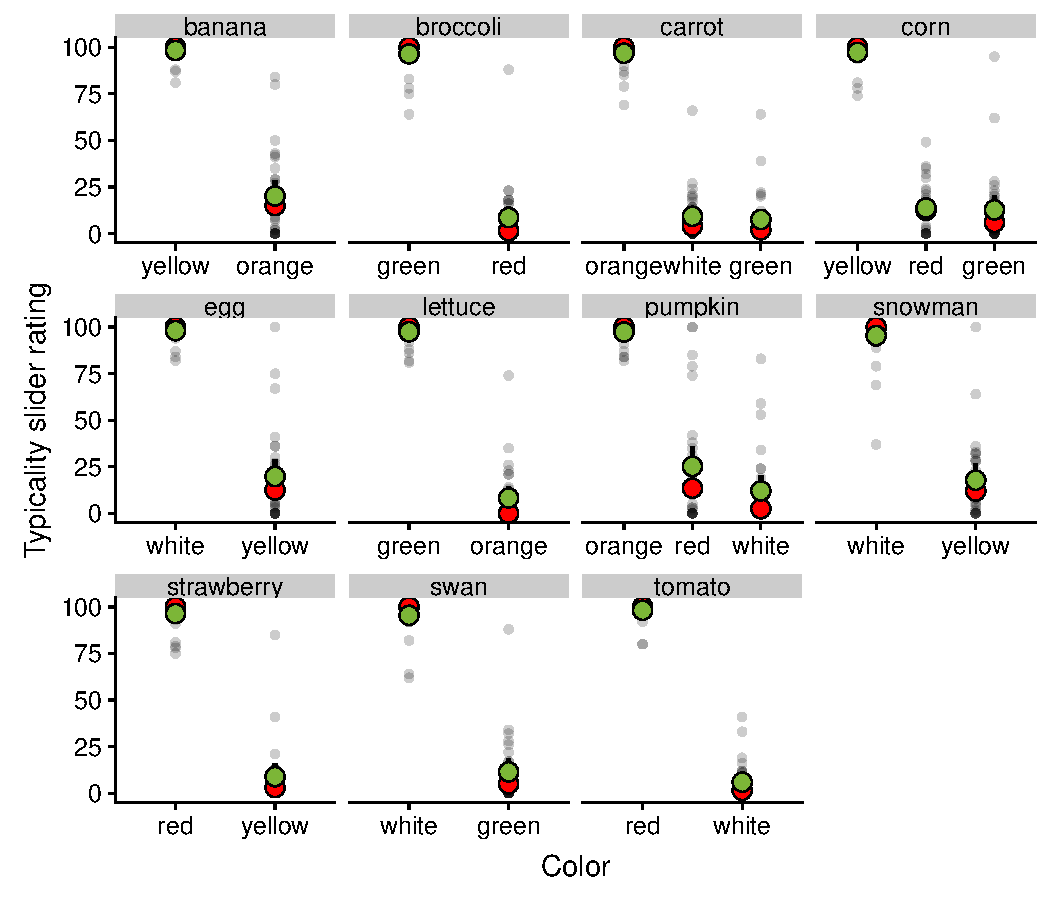
\includegraphics[width=0.9\linewidth]{img/norming3_results.pdf}
	\caption{Typicality ratings for differently colored instances of the same object. Higher values indicate higher typicality. Individual data points are in gray, means in green and medians in red.}
	\label{fig:norming3results}
\end{figure}

As shown in Figure \ref{fig:norming3results}, there generally was a clear distinction between the typical and atypical instances for each object. 
Of the three items that were normed in two atypical colors (carrot, corn, and pumpkin), the red and white pumpkin showed the biggest difference. Therefore, we chose the white over the red pumpkin, and, following from that, the green carrot and red corn as atypical instances. 
Finally, even though the egg and snowman received similar ratings for their atypical instance, the white egg is rated slightly more typical than the depiction of the white snowman.

However we have to note that even though the orange banana is predominantly rated below 50, it is still not as atypical as other items. This might be due to the high similarity between the colors yellow and orange.

\section{Norming for free production}
\label{freeprodnorming}

% Goal: Are the image depictions we chose nameable, the way we intended?

% Task: "What is this?"

% free production

% 31 trials (22 cd -- each participant saw one instance of each object at random, i.e., either typical or atypical; 20 non-cd)

% Results: swan is often called a goose; two people identified the white carrot as parsnip

% \subsection{Final stimuli selection}

% In the end, we have 10 objects, each occurring in a typical and atypical color.
% Items can occur in the colors yellow, red, green, orange and white. Each color occurs twice as typical and twice as atypical. This counterbalance aims to reduce artifacts of salience such as red is generally more salient as a warn signal \ek{ref?} and blue is highly atypical for most objects. A full list of stimuli can be found in table \ek{add table and reference}.

Finally, we normed the stimuli chosen from the typicality norming study as to whether those depictions are nameable as intended.

\paragraph{Participants}
We recruited 50 participants over Amazon's Mechanical Turk. We restricted participation to workers within the US and a previous Hit approval rate of at least 97\%. The study took about 5 minutes and we paid \$1.10 for participation. 

\paragraph{Materials and procedure}
As stimuli, we used the objects and depictions selected from the typicality norming study, which was almost identical to the complete final set. The only redundancy at this point was the egg vs. snowman stimulus. 

Participants saw each object exactly once and its typicality was randomized, resulting in 11 critical trials. This was done to prevent convergence effects on a label when the object occurred the second time (e.g., \cite{Clark:1986}). Each participant additionally completed 20 filler trials, where they saw non-color-diagnostic objects.

\paragraph{Analysis and exclusions}
Three participants were excluded because they indicated that they did the experiment incorrectly or were confused, and another three participants because they used non-anticipated utterances in more than 1/3 of the trials.

\paragraph{Results}

\begin{figure}
	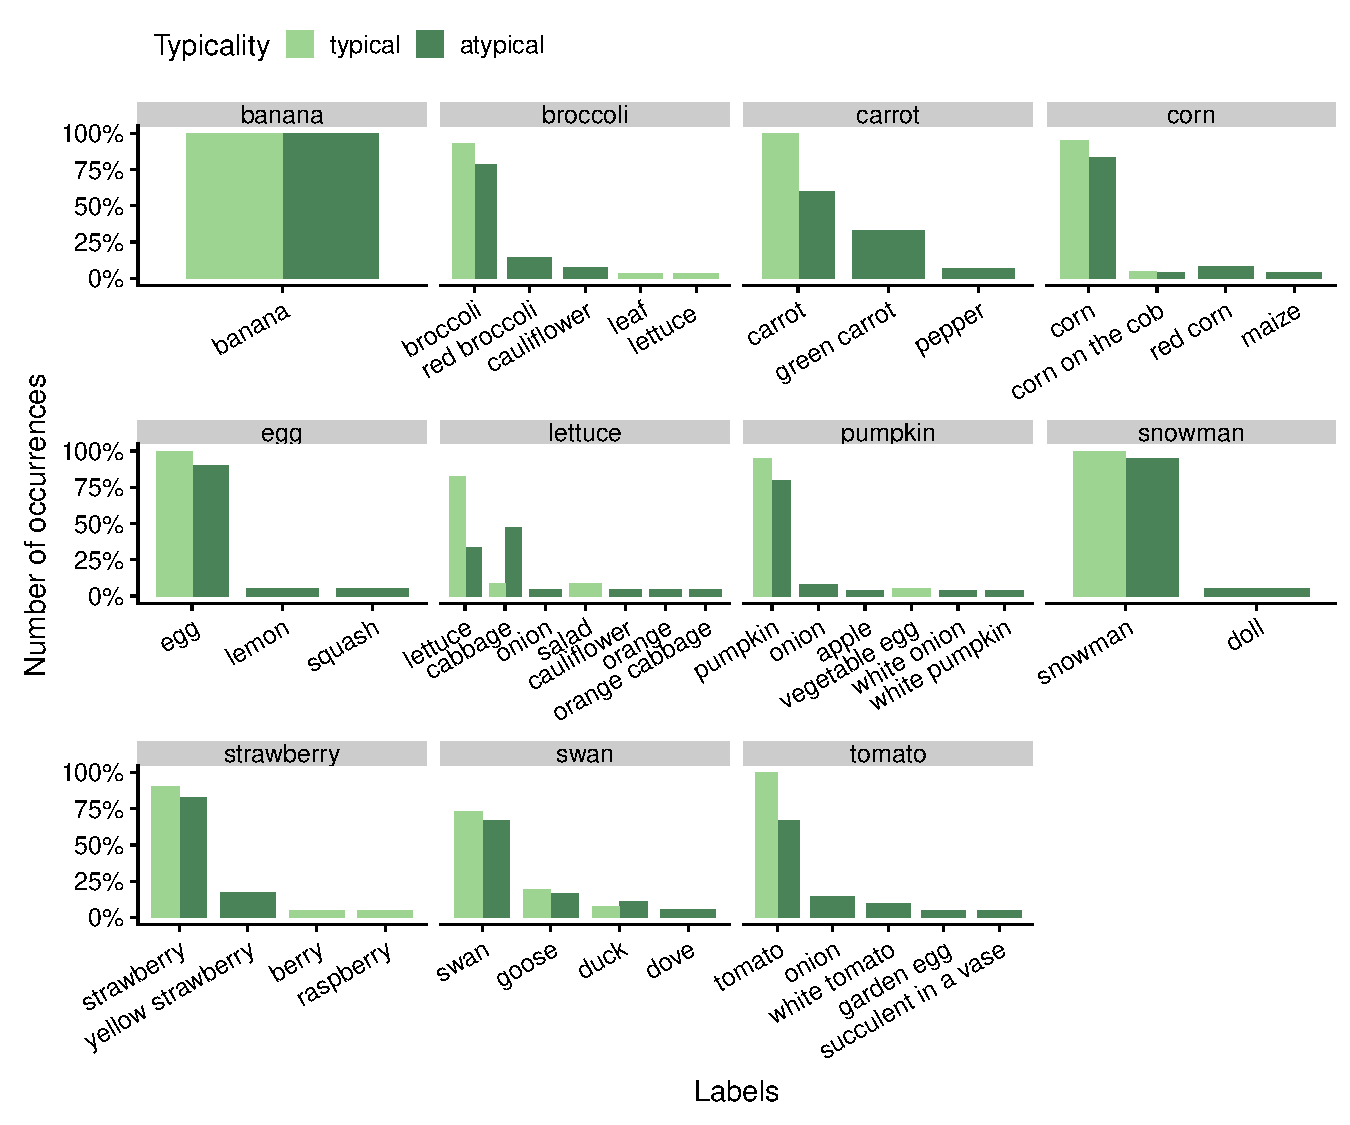
\includegraphics[width=0.9\linewidth]{img/norming4_results.pdf}
	\caption{Labels produced for each item in a free production experiment for all remaining stimuli. Labels produced for typical items are in light green, labels produced for their atypical counterparts in dark green.}
	\label{fig:norming4results}
\end{figure}

As the results in Figure \ref{fig:norming4results} show, participants generally gave the same label to both the atypical and typical instance. This supports the final stimulus selection. 
Since egg and snowman were both equally nameable, we chose the egg as the typical white instance due to its size compatibility with the other items. 

There are three stimuli that are slightly less clearly nameable than the others: the atypical lettuce is often called \textit{cabbage}, the swan is sometimes mistaken for a goose and the white carrot has been mislabeled as a parsnip by two participants. However we accept these deviations as negligible.

Lastly we observed that even in this highly simplified setup with written free text input, participants sometimes produced the color term spontaneously, but only for the atypical items (for example for the green carrot, red corn, and white tomato).



% \subsection{Norming for multiple choice}


\section{Conclusion}

\begin{figure}
	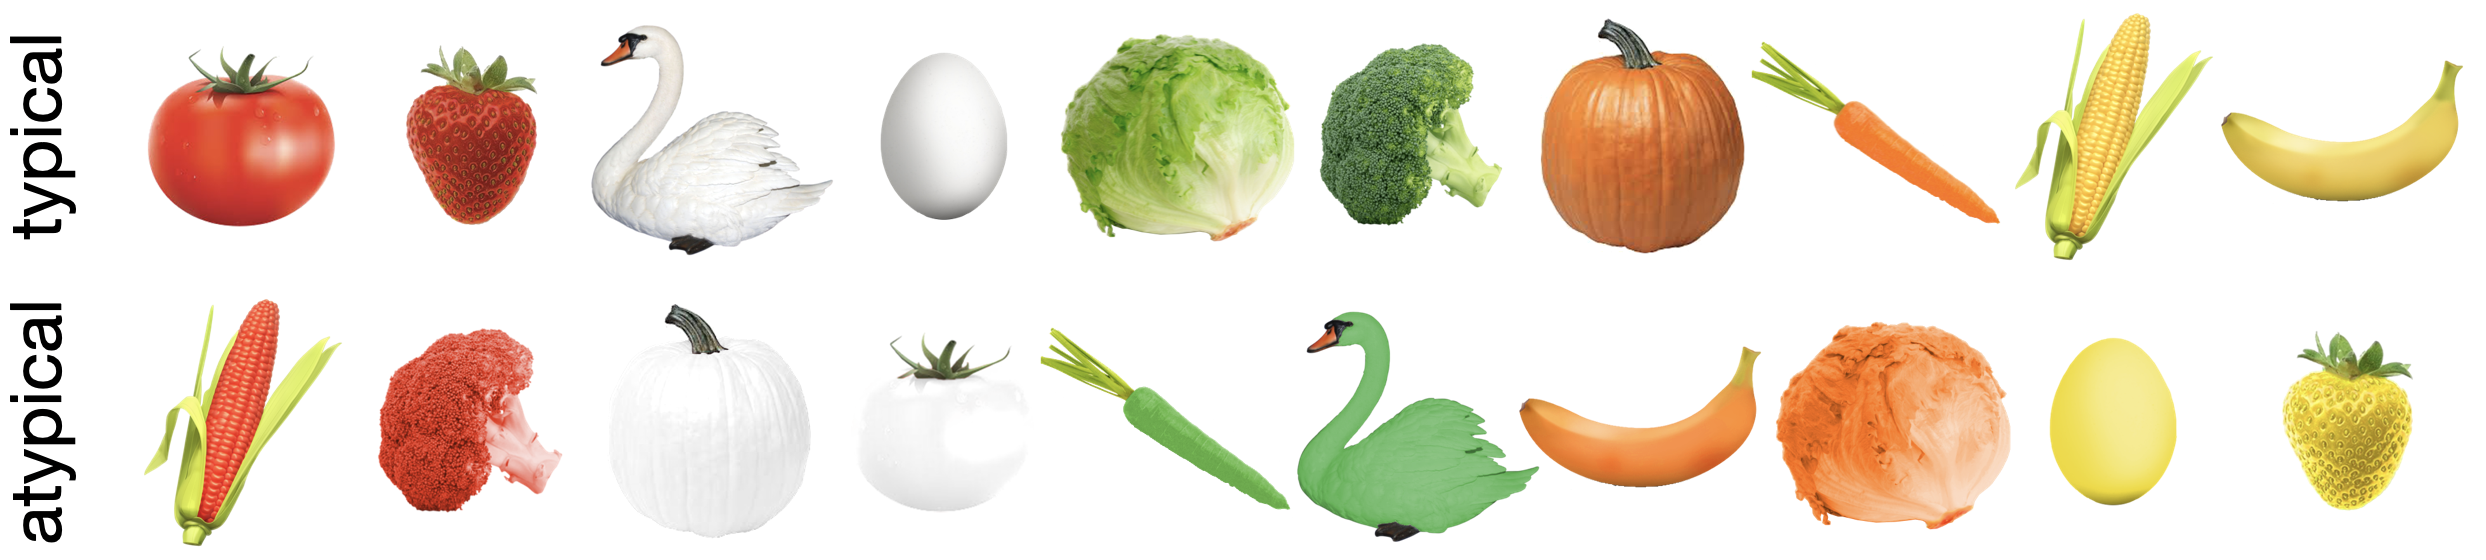
\includegraphics[width=0.6\linewidth]{img/finalstimuli.png}
	\caption{Final set of stimuli, ordered by color and typicality. Each object occurs in a typical and atypical color.}
	\label{fig:finalstimuli}
\end{figure}

In the end, the final set of stimuli comprises 10 objects, each occurring in a typical and atypical color.
Items can occur in the colors yellow, red, green, orange and white. Each color occurs twice as typical and twice as atypical. The objects are \textit{banana, broccoli, carrot, corn, egg, lettuce, pumpkin, strawberry, swan,} and \textit{tomato}. The full set of stimuli is displayed in Figure \ref{fig:finalstimuli}.



\bibliography{QP1}

\vfill
\pagebreak

\end{document}

%
% Please see the package documentation for more information
% on the APA6 document class:
%
% http://www.ctan.org/pkg/apa6
%





















% \section{Experiment: Comprehension} \label{experiment}

% \subsection{Method}

% \paragraph{Participants}
% We recruited 80 participants over Amazon's Mechanical Turk, 40 for each color competitor typicality manipulation. The study took on average 7 minutes and each of them were paid \ek{...} for their participation. We restricted participation to workers with IP addresses in the US and a approval rate of previous work above 97\%.

% \paragraph{Procedure}
% This experiment is a one-player adaptation of the production study explained in \ek{ref to section} and follows the design of an incremental decision task \ek{cite Qing}. participants were put into the listener role of the reference game. That means, they needed to identify which object was the target given a referring expression placed above the grid. Crucially, they do not observe the complete referring expression at once, but instead the utterance is gradually revealed. After new information is revealed, participants are required to make their best guess onto which object is the most likely target. The choices had to be made prior any disambiguating information (after observing "Click on the"), after observing an adjective ("Click on the yellow") and after observing the fully disambiguating noun ("Click on the yellow banana!"). The clicks before information are observed are useful to determine whether there are already strong priors in item selections, even before any information were observed. The clicks after revealing the adjective are the critical clicks that will affect our interpretation of inferences drawn from the adjective. After observing the noun there is only one possible referent left. These clicks are used as attention checks.

% Participants completed 55 trials in total, 20 of which were critical trials and 35 were fillers. The filler trials were supposed to ensure that participants perceive the referring expressions as being generated by a natural speaker. Firstly, all target trials are color modified utterances. To avoid that participants learn that the color modifier is always part of the referring expression, we need utterances that only have the bare noun. Second of all, we need to make sure that targets are not logically derivable. In a context such as \ek{Fig ref!}, the target can be determined by reasoning about the distractor choice. The target is the only object that shares the type (i.e., banana) with a distractor and its color (i.e., yellow) with another distractor. One can then derive that the object that is being distracted from will be the target. This regularity could also be learnt over the time course of the experiment. The filler trials therefore need to introduce primarily unmodified referring expressions that target other objects in the display. The exact trial structure is summarized in table \ref{tab:trialstructure}.

% \begin{table}[]
% 	\begin{tabular}{llll}
% 	\textbf{trial type} & \textbf{number} & \textbf{utterance} & \textbf{referent}           \\
% 	critical            & 20              & modified           & target                      \\
% 	filler              & 5               & unmodified         & color competitor (typical)  \\
% 	filler              & 5               & modified           & color competitor (atypical) \\
% 	filler              & 5               & modified           & contrast                    \\
% 	filler              & 20              & unmodified         & distractor (typical)       
% 	\end{tabular}
% 	\vspace{2mm}
% 	\caption{Overview of the trial structure for the comprehension study.}
% 	\label{tab:trialstructure}
% \end{table}

% Before participants proceeded to the main trials, they had to complete four practice trials constructed from the speaker perspective. In the speaker role, they saw a grid of four non-color diagnostic objects, one of which was marked as the target by a green border surrounding it. They were then asked to refer to the object such that a second player could identify it. The practice trials were introduced to familiarize the participants with the task.

% The main trials were randomized with one restriction: Trials in which we expect a color modifier to be superfluous or even misleading only occurred after the 15th trial. These were contexts where there was no contrast and either both target and color competitor typical objects, or the target typical while the color competitor was atypical. This measure should minimize the risk that participants perceive the "utterance generator" as unnatural.

% \paragraph{Materials}

% \ek{add choice of contexts (i.e., one per color,...); clarify what is within and between-subject manipulation with rationale}

% The stimuli were the same as in the production study.

% \paragraph{Data Preprocessing and exclusion}

% We excluded participants who indicated that they did the Hit incorrectly or were confused (7), who indicated that they had a native language other than English (4), who gave more then 20\% erroneous responses (2) and who did the Hit multiple times (1). Overall, we excluded 14 out of 80 submissions (17.5\%). An erroneous response is defined as a click to a non-target object after observing the fully disambiguating noun, i.e., participants are excluded who selected the wrong final object more than 11 times.

% \subsection{Results}

% \section{Discussion}